\documentclass{article}
\usepackage{graphicx}
\begin{document}

\author{Andrew Bartnof,for RMI}
\title{Difference-in-Difference Study for GGRF}
\date{\today}
\maketitle

\section{Introduction}

This paper documents my difference-in-difference (\emph{DiD}) analyses for the GGRF insurance project, in which I attempt to quantify the impact of a green energy project on a neighborhood's home appreciation rates.
I present a mixed-effects model in the main part of this paper.
In the appendix, I present another model, which uses a more conventional two-way fixed-effect DiD schema.

\section{Brief Background}

If green energy projects (eg solar farms and wind turbines) are built near residential areas, these projects can impact local home values, lowering the rate at which they appreciate vis-\`a-vis homes in other areas.
This gives home-owners an incentive to resist green projects in their neighborhoods, even if they support green projects in general.

We want to quantify this potential relative change in the rate in which homes appreciate near green energy projects, so that we can help to develop a new kind of financial project; a parametric risk insurance payout for home-owners near green energy projects.
The idea is that, for a limited amount of time, while the green energy projects artificially depress local homes' values, any home-owner that sells their house can be compensated for this drop in home-value.


\section{Data}

Naturally, there are a few dimensions we'd like to better understand-- do all green energy projects lower the rates at which homes appreciate? how far need a house be from a project before its value is impacted? and how long does this change in home value endure?
This is a rather 'cheap-and-cheerful' analysis using readily-available datasets, so I'll attempt to answer these, while making sensible assumptions where necessary.

In this paper, I'll  refer to homes that are near green energy projects as \textbf{manipulation} homes, and homes that are not near green energy projects as \textbf{control} homes.

I use three key datasets:

\subsection{Zillow Home Prices}
This dataset lists the home prices for 26,344 zip-codes, between the years 2000 and 2024.
This was collected before I jumped on the GGRF project so I can't give much more insight into it.

\subsection{Large-Scale Solar Photovoltaic Sites}
The solar dataset\footnote{Fujita, K.S., Ancona, Z.H., Kramer, L.A. et al. Georectified polygon database of ground-mounted large-scale solar photovoltaic sites in the United States. Sci Data 10, 760 (2023). https://doi.org/10.1038/s41597-023-02644-8} lists the locations and years of operation of thousands of large-scale solar photovoltaic sites.
Note that Ben Hoen is an author of both this dataset and the turbine dataset.

\subsection{Wind Turbines}
This dataset\footnote{
Rand, J.T., Kramer, L.A., Garrity, C.P. et al. A continuously updated, geospatially rectified database of utility-scale wind turbines in the United States. Sci Data 7, 15 (2020). https://doi.org/10.1038/s41597-020-0353-6} lists the locations and years of operation of thousands of wind turbines.

\subsection{Data Notes}
Each observation in the solar and turbine datasets is represented as a polygon in a shapefile.
The Zillow file commits us, however, to using zip-codes as our finest geographic granularity.
Consequently, I assign each solar and turbine project to a single zip-code. 
Any homes that share a zip-code with a green project are considered manipulations.
(We'd prefer not to say that a home either \emph{is}, or \emph{isn't}, near a solar project as if it's a binary metric, but it'll do.)

I also round all dates to the year.
If there are multiple home values noted in a given zip-code within this year, I take the median home price.

\section{Mixed-Effects Model}

The formula for our mixed-effects model looks like this:
\begin{verbatim}
rate of home appreciation ~ 
\end{verbatim}
\begin{verbatim}
year + solar_manipulation + turbine_manipulation + (1|zip_code)
\end{verbatim}

\textbf{Dependent variable}
\begin{itemize}
\item The rate of home appreciation is calculated as: \emph{(current home price - last year's home price) / (last year's home price).}
\end{itemize}

\textbf{Fixed effects}
\begin{itemize}
\item Year: the calendar year, represented as an unordered factor. This allows us to represent general market fluctuations (eg the Great Recession) easily.
\item Solar manipulation: if a zip code ever had a solar plant built there, we encode the zip-code each year as one of the following:
	\begin{itemize}
	\item Construction: if only one solar plant is built in this zip-code, then 'construction' is synonymous with 'year of operation'. If multiple solar plants are built in this zip-code, this represents the duration between the first plant's year of operation and the last plant's year of operation. 'Construction' indicates that we have faith that during this time period, workers and trucks were around.
	\item -5:-1: Years prior to year of first plant's operation
	\item 1:5: Likewise, years after last plant's operation
	\item Censored: if we are more than five years before construction, or less than five years after, construction in a zip-code
	\item Control: a zip-code that never gets a solar project
	\end{itemize}
\item Turbine manipulation: encoded exactly like solar manipulation
\end{itemize}
\textbf{Random effects}
\begin{itemize}
\item Zip-code: here, I model all zip-codes as random intercepts. This is common practice in models that have repeated measures per subject; this compensates for the mean difference in home appreciation in each zip-code
\end{itemize}


\subsection{Goodness-of-Fit Metrics}
In order to verify whether it's even sensible to try to calculate the impact of green energy projects, we also fit a null model, which omits turbine manipulation and solar manipulation.
This means that the null model's formula is:
\begin{verbatim}
change in home price v. last year ~ year + (1|zip_code)
\end{verbatim}
.

An ANOVA comparing these two models indicates that the full model is statistically significant (see figure \ref{anova}).
This indicates that it the turbine and solar manipulations are statistically significant.

\begin{figure}[h]
\centering
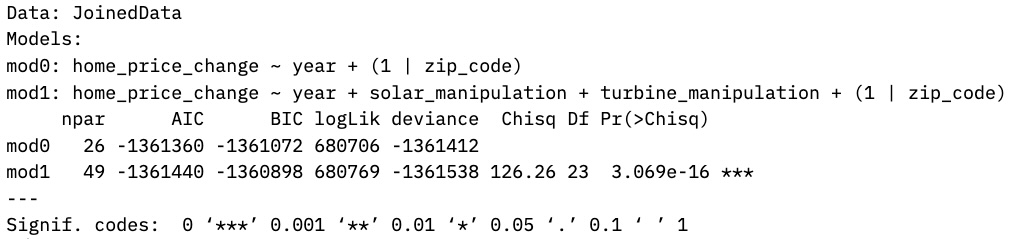
\includegraphics[width=0.9\linewidth]
{lmer_mod_anova.jpg} 
\caption{The full regression model is statistically significant, compared to the null model which omits green energy projects.}
\label{anova}
\end{figure}

The unadjusted intra-class correlation (ICC) is 0.011, which is quite low.
A high ICC would that a lot of the variance that is explained in the full model is done by the random-effects.
Rather, our fixed effects are explaining a lot of the variance-- and the effects we're trying to model are all fixed-effects.

\subsection{Estimates}

The fixed effects can be seen in figure \ref{fixef_general} and figure \ref{fixef_manipulation}, but they are listed below in their entirity.
Note that any variable whose 95\% CI includes 0.0 can plausibly be said to be negligible.

\begin{table}[]
\begin{tabular}{llll}
\textbf{Variable}                 & \textbf{Estimate} & \textbf{2.5\%} & \textbf{97.5\%} \\
(Intercept)                       & 0.053             & 0.047          & 0.058           \\
year2002                          & 0.015             & 0.013          & 0.016           \\
year2003                          & 0.014             & 0.013          & 0.015           \\
year2004                          & 0.021             & 0.02           & 0.023           \\
year2005                          & 0.047             & 0.046          & 0.049           \\
year2006                          & 0.05              & 0.049          & 0.052           \\
year2007                          & -0.013            & -0.014         & -0.012          \\
year2008                          & -0.071            & -0.072         & -0.069          \\
year2009                          & -0.131            & -0.132         & -0.13           \\
year2010                          & -0.116            & -0.117         & -0.115          \\
year2011                          & -0.09             & -0.091         & -0.089          \\
year2012                          & -0.097            & -0.098         & -0.096          \\
year2013                          & -0.029            & -0.031         & -0.028          \\
year2014                          & 0.005             & 0.004          & 0.006           \\
year2015                          & -0.012            & -0.013         & -0.01           \\
year2016                          & 0.001             & -0             & 0.002           \\
year2017                          & -0.014            & -0.016         & -0.013          \\
year2018                          & -0.003            & -0.004         & -0.002          \\
year2019                          & -0.003            & -0.004         & -0.002          \\
year2020                          & -0.006            & -0.008         & -0.005          \\
year2021                          & 0.055             & 0.054          & 0.057           \\
year2022                          & 0.082             & 0.081          & 0.083           \\
year2023                          & 0.015             & 0.014          & 0.016           \\
year2024                          & -0.03             & -0.031         & -0.029          \\
solar\_manipulation-2             & -0.001            & -0.004         & 0.003           \\
solar\_manipulation-3             & -0.001            & -0.005         & 0.002           \\
solar\_manipulation-4             & -0.002            & -0.005         & 0.002           \\
solar\_manipulation-5             & -0.003            & -0.007         & 0.001           \\
solar\_manipulation1              & 0.004             & 0              & 0.007           \\
solar\_manipulation2              & 0.004             & 0              & 0.007           \\
solar\_manipulation3              & 0.006             & 0.003          & 0.01            \\
solar\_manipulation4              & 0.01              & 0.006          & 0.014           \\
solar\_manipulation5              & 0.009             & 0.005          & 0.013           \\
solar\_manipulationCensored       & 0.004             & 0.001          & 0.006           \\
solar\_manipulationConstruction   & 0.003             & -0             & 0.006           \\
solar\_manipulationControl        & 0.006             & 0.001          & 0.011           \\
turbine\_manipulation-2           & 0                 & -0.006         & 0.007           \\
turbine\_manipulation-3           & 0                 & -0.006         & 0.007           \\
turbine\_manipulation-4           & 0.001             & -0.006         & 0.007           \\
turbine\_manipulation-5           & 0.001             & -0.006         & 0.008           \\
turbine\_manipulation1            & -0.001            & -0.007         & 0.004           \\
turbine\_manipulation2            & -0.004            & -0.01          & 0.002           \\
turbine\_manipulation3            & -0                & -0.006         & 0.006           \\
turbine\_manipulation4            & 0                 & -0.006         & 0.006           \\
turbine\_manipulation5            & -0.003            & -0.009         & 0.004           \\
turbine\_manipulationCensored     & 0.003             & -0.002         & 0.008           \\
turbine\_manipulationConstruction & 0.002             & -0.003         & 0.007          
\end{tabular}
\end{table}

Do note that while this model gives quite sensible estimates, we suffer from a relatively low sample size for a model of this complexity.
We have 412,303 observations in our control group, and only 58,839 in our manipulation group.
For this reason, this model was slightly rank-defficient.
(One notable missing value is turbine manipulation for the year just before operation.)

\begin{figure}[h]
\centering
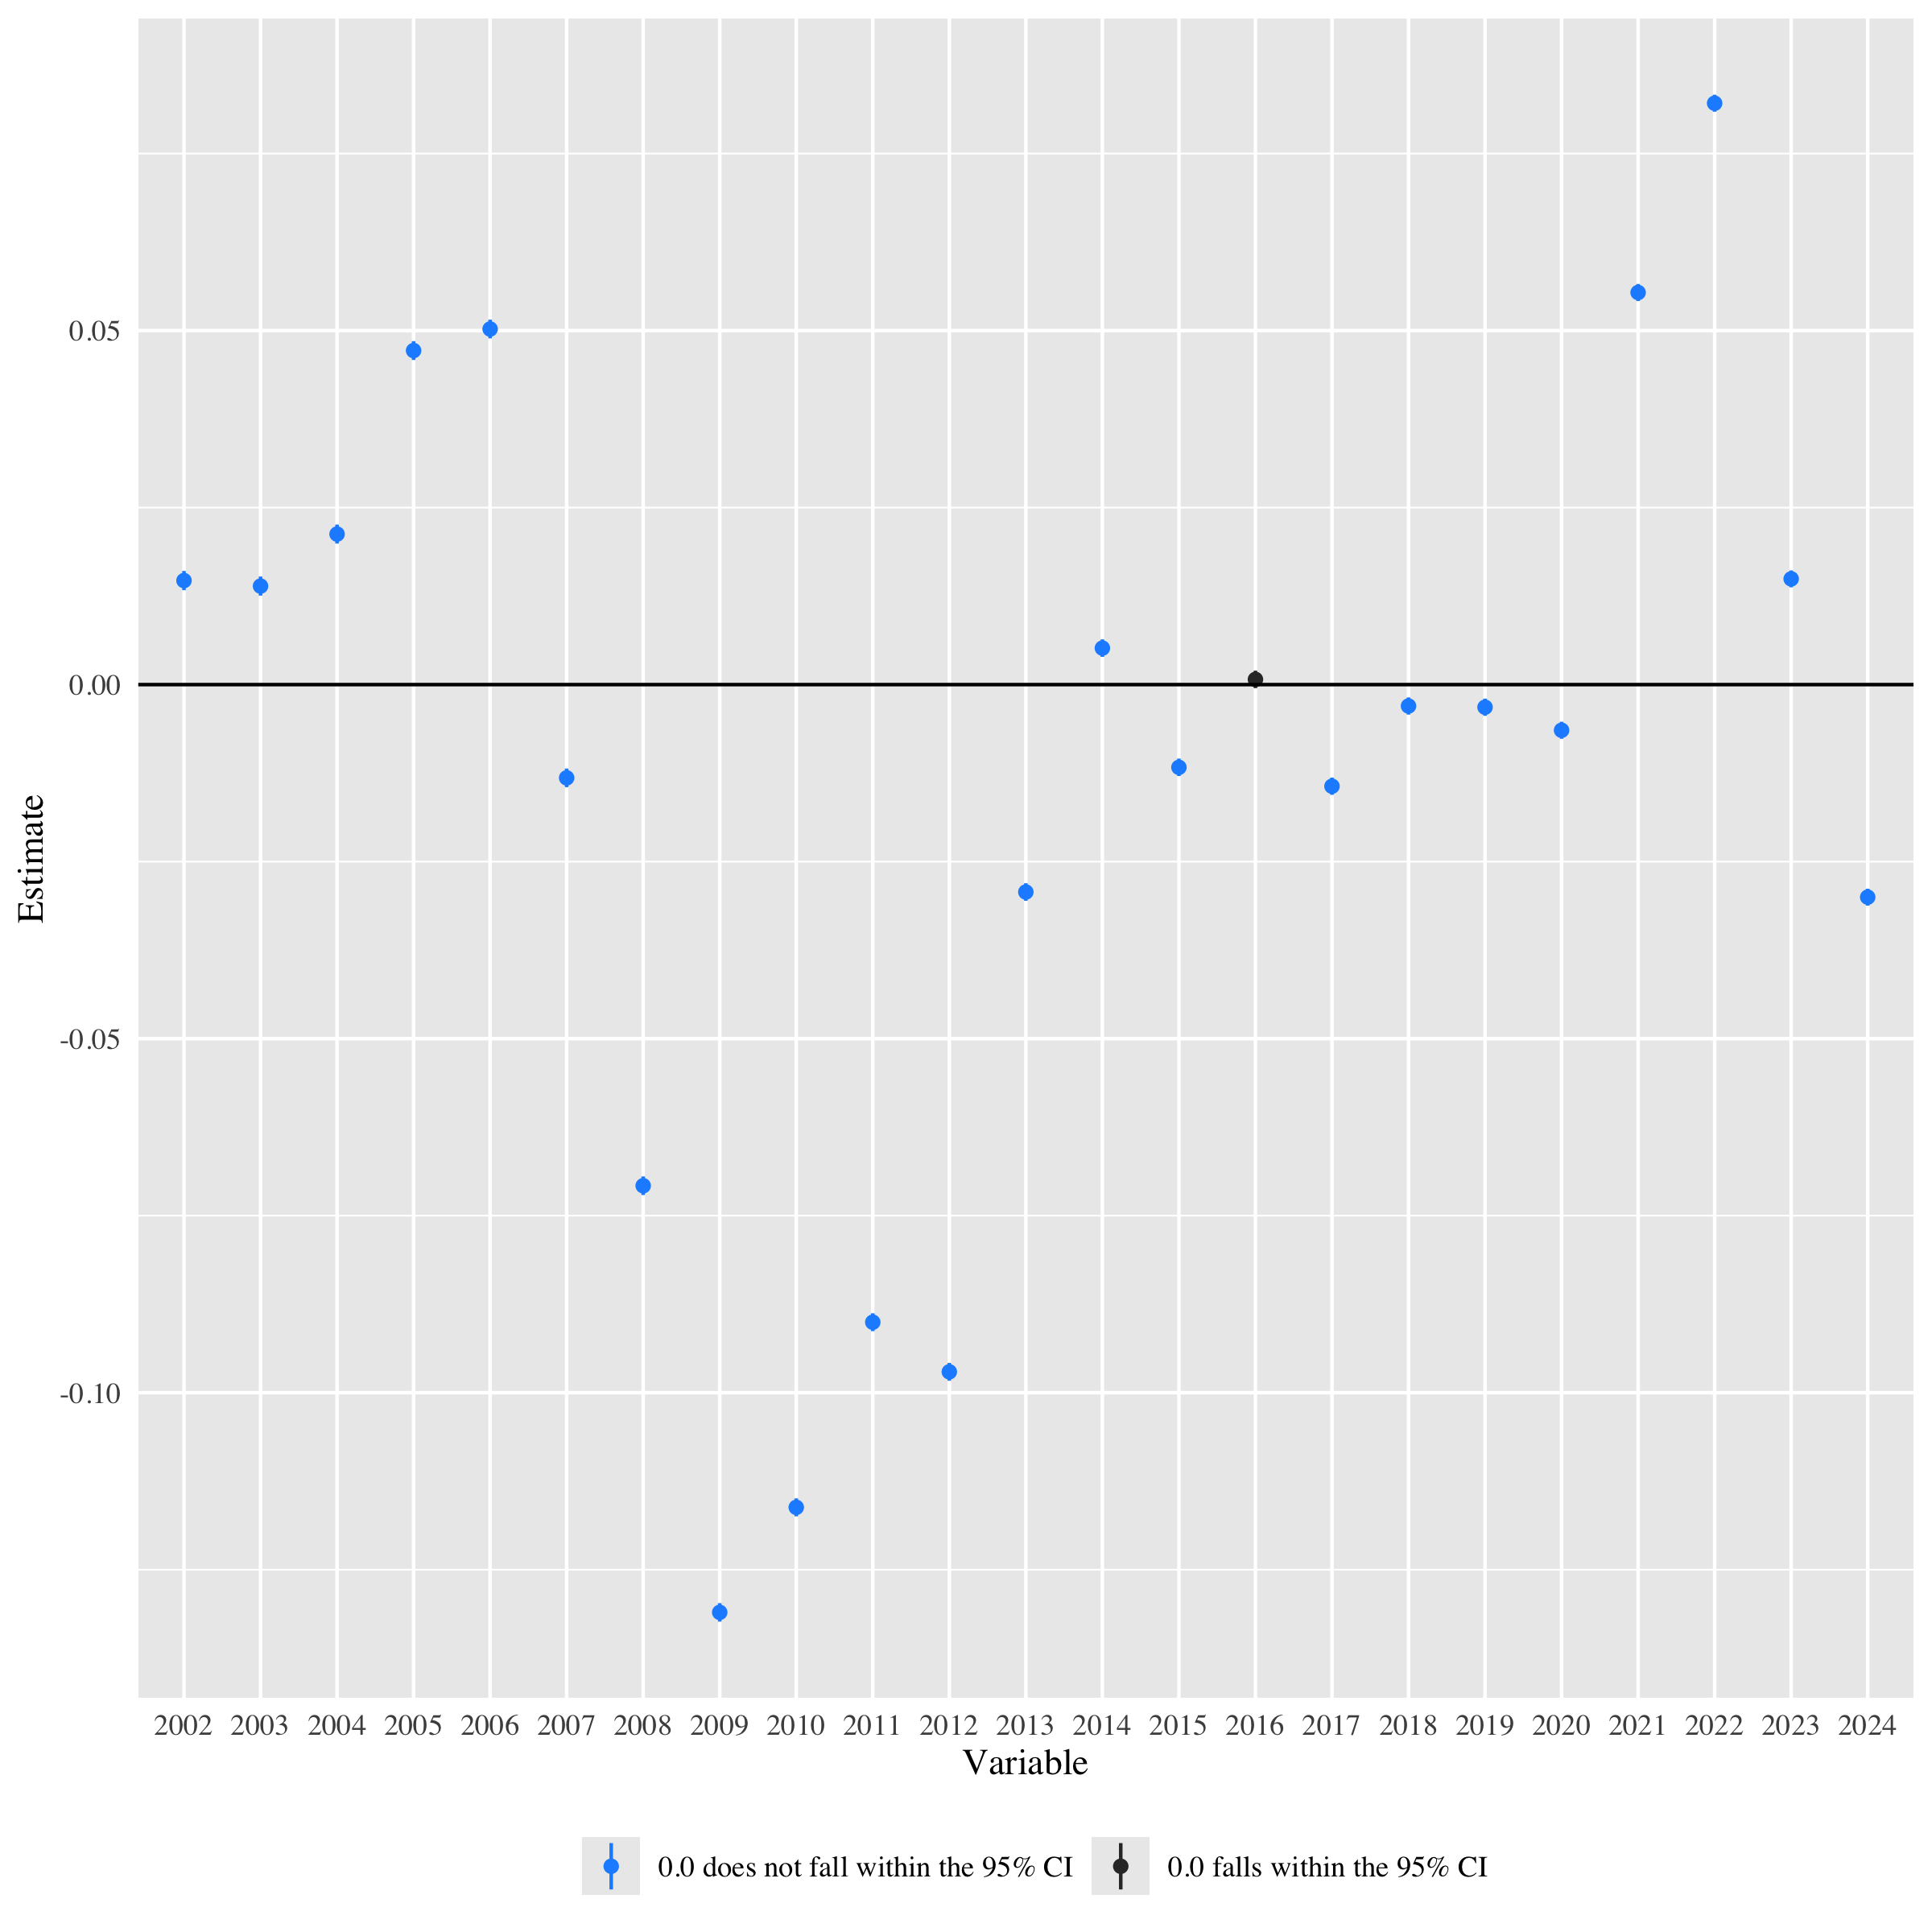
\includegraphics[width=0.9\linewidth]
{fixef_general.png} 
\caption{Some of the fixed effects from the second study.}
\label{fixef_general}
\end{figure}

\begin{figure}[h]
\centering
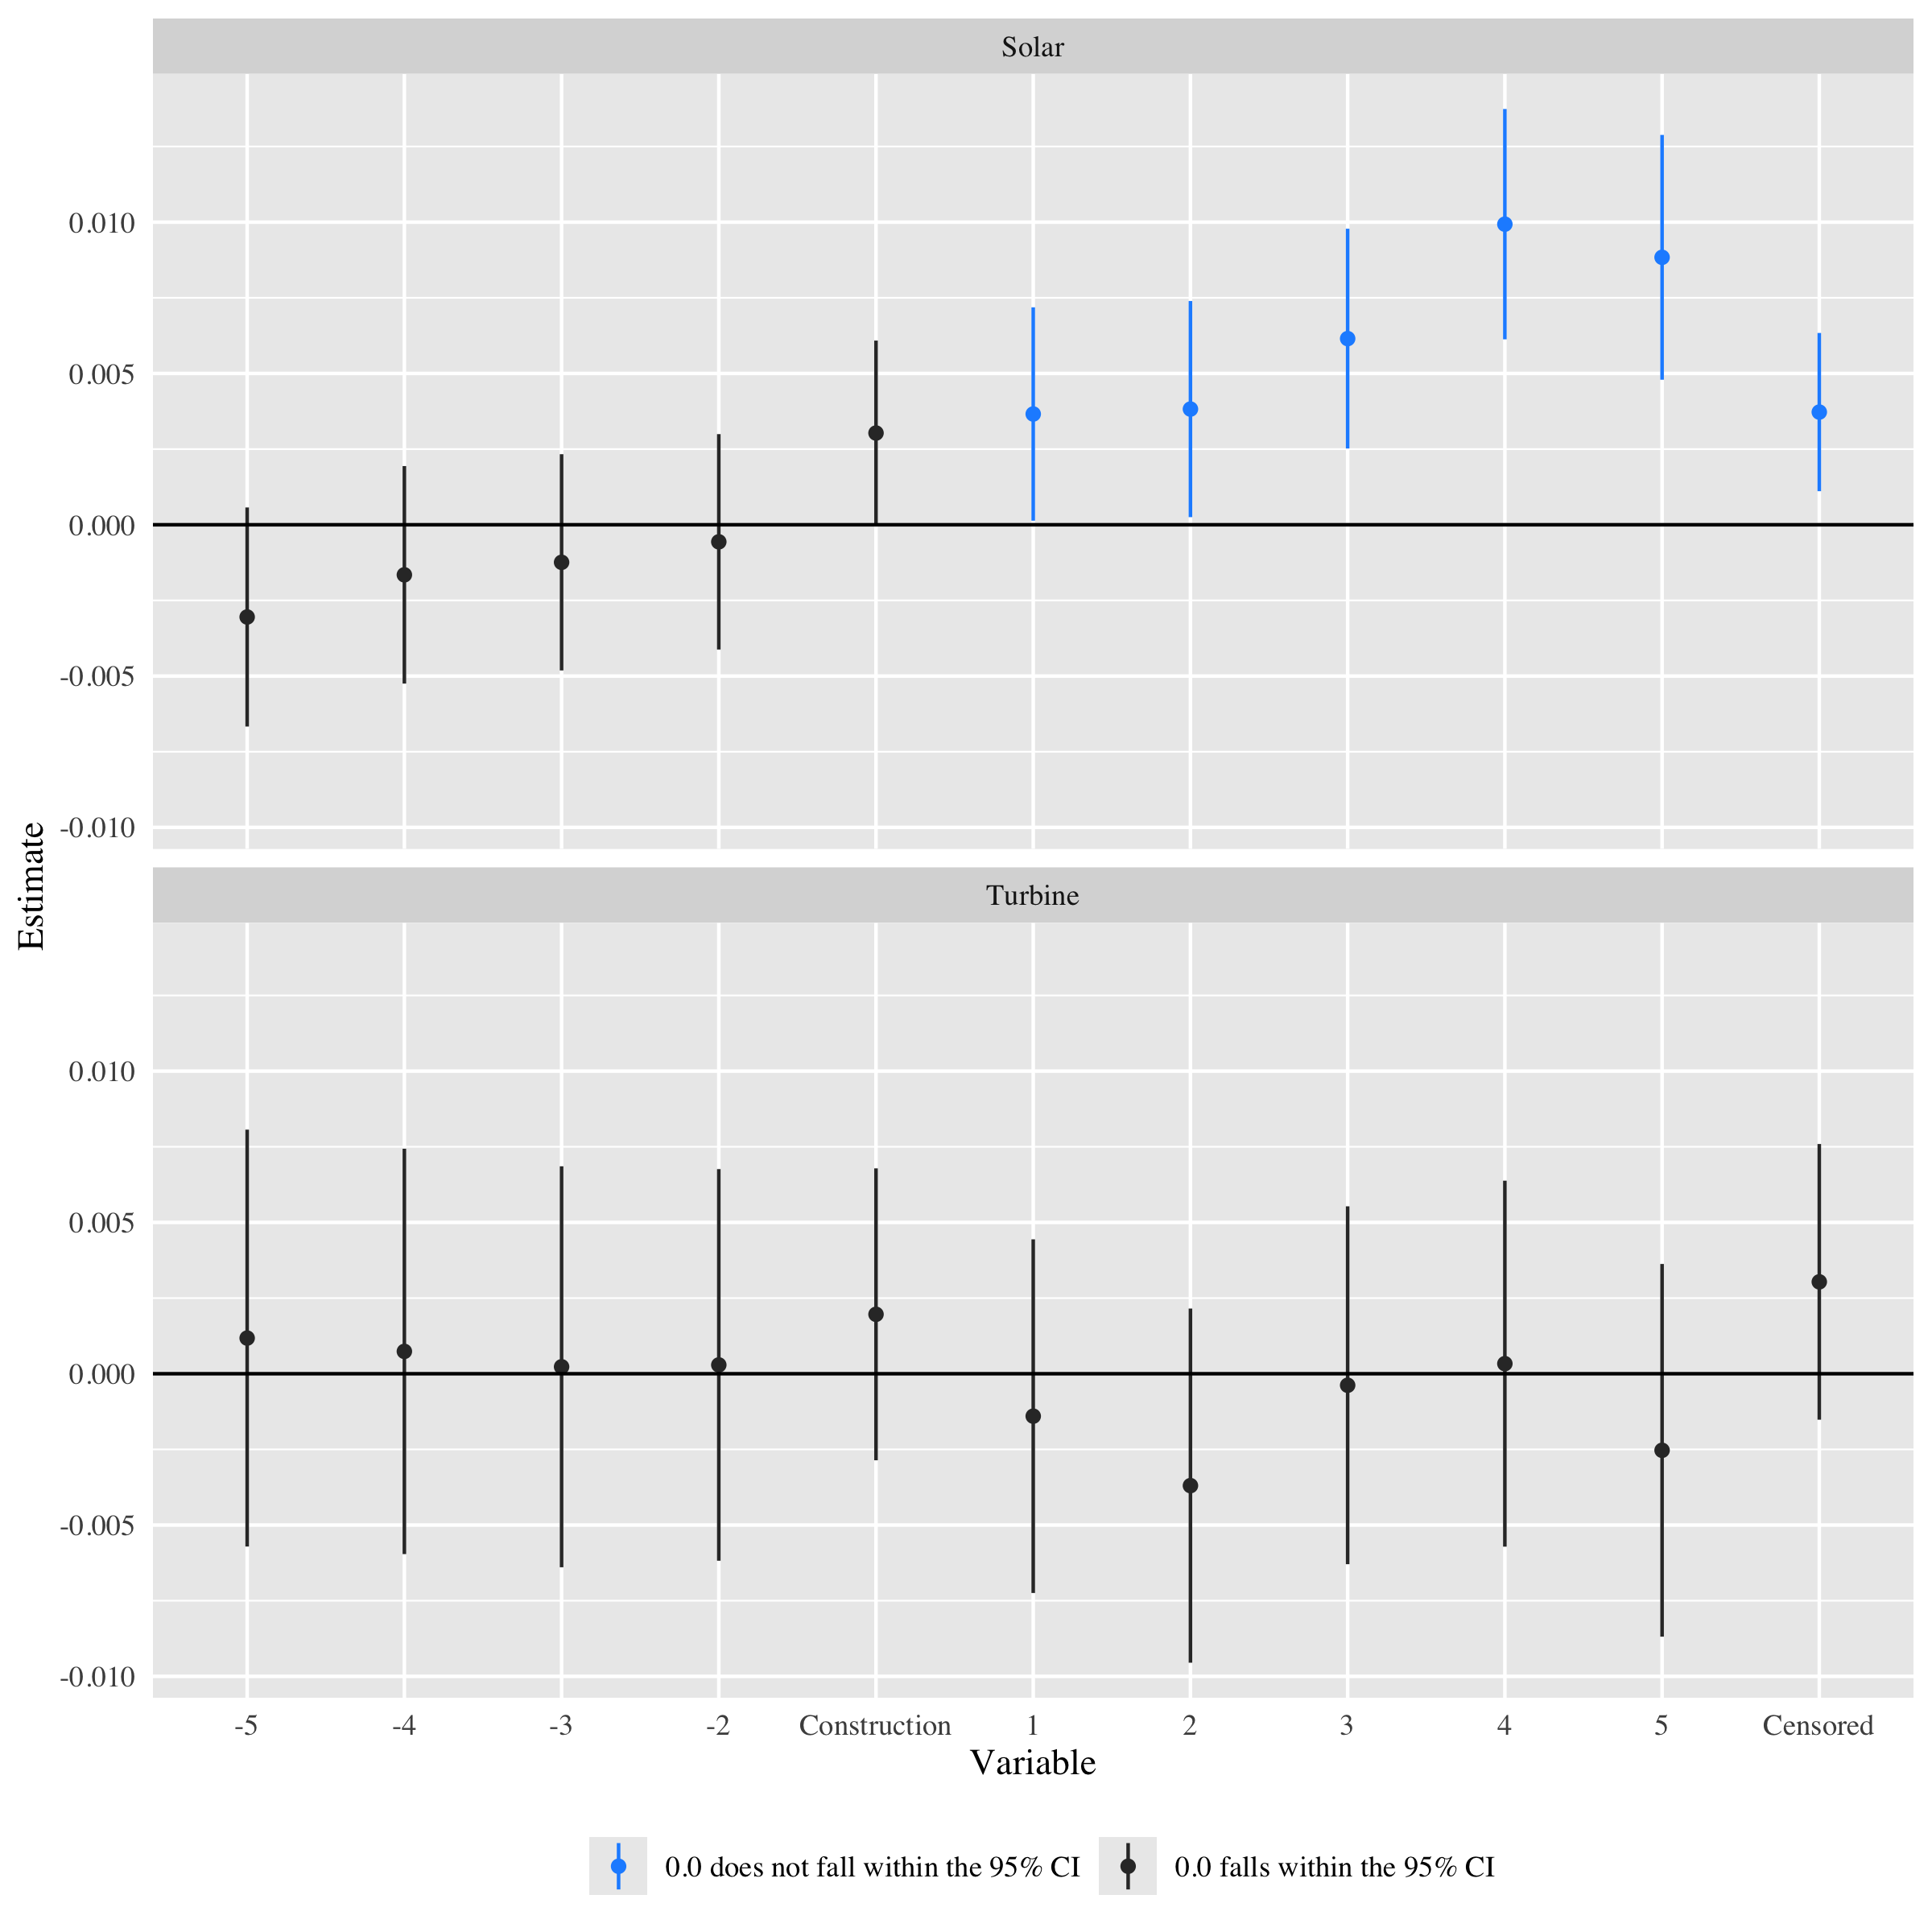
\includegraphics[width=0.9\linewidth]
{fixef_manipulation.png} 
\caption{The rest of the fixed effects from the second study.}
\label{fixef_manipulation}
\end{figure}

Figure \ref{fixef_general} shows the annual intercepts for overall home appreciation in the national market.
Figure \ref{fixef_manipulation} shows what happens when solar and turbine projects are built in a zip-code.
Bearing in mind that \emph{these fixed-effects don't reflect home prices, but instead, the rates at which home-prices change given different situations}, I interpret these in the following way:
\begin{itemize}
\item We can posit that any fixed-effect whose 95\% confidence interval includes zero does not significantly differ from no effect at all. 
Consequently, we can't really glean too much from  most of the trends that we see in the solar and turbine diagram (diagram \ref{fixef_manipulation.png}), because their CIs generaly contain zero. 
On the other hand, our dataset is kind of small for this kind of model, and highly imbalanced. 
We can see how small the dataset is because our model is slightly rank-defficient.
We can see evidence of how imalanced the dataset is in the very slim 95\% CIs in the yearly fixed-effects, when compared to the large ones in the manipulations; this might be because we have so many more observations in our control set than in our manipulation set. 
I suggest we cautiously try to make sense of the manipulation trends, while acknowledging that without a larger dataset, our conclusions are generally speculative.
\item The only estimates whose CIs don't include zero are the solar estimates, in the years after the construction is done, and in the periods before and after five years away from construction ('censored'). 
Given the means to follow-up on this, I would like someone on our team to test the hypothesis that this rate of change that is positive vis-a-vis the baseline rate of change reflects the home-values in these areas quickly returning to what they would be if the solar plant had never been installed.
That is to say, I don't hypothesize that areas with solar plants have higher property values than areas without; I just think that the rate of change is positive in order to bring us back closer to national norms, once the construction is over. 
(The fact that the 'censored' value is positive could challenge this hypothesis. Positive censored estimates AFTER construction jibes with my theory; positive censored values BEFORE construction challenge it. But in a model that is already rank-defficient, I can't really slice and dice our data much more to explore this.) 
\item Homes that are near construction sites appreciate in value slower than homes in control groups, which makes sense to me.
\item I wonder if property values for zip-codes with turbines never fully rebounds after construction is over, because turbines make a bit of noise and are highly visible.
\end{itemize}


\section{Appendix}

I think that the previous model is my best attempt to model this data.
However, a classic Difference-in-Difference comparison isn't done with a mixed-effects model-- it's done with a two-way fixed-effects model.
So, in order to honor convention, I model that as well.
I include it in the appendix for your edification-- so you can see its results, and also, why I take issue with this model.

This model simplifies the previous model by simply asking if the rate of home appreciation changes over time, differently in neighborhoods that DO have solar/turbines developed there versus in neighborhoods that DON'T.

So, for any target year, I note all of the zip-codes that had a solar facilities come online in that target year.
I track the rate of home appreciation in those (manipulation) zip-codes for five years before, and five years after, the plants came online.
I then compare this rate of appreciation to the national rate of home appreciation in zip-codes that had neither solar nor turbine facilities built, ever (control).
Once again, rate of home appreciation is defined as:
\noindent\textit{(current home price - last year's home price) / (last year's home price). }

And once again, I'd do this once with zip-codes that had solar facilities built, and then again with zip-codes that had turbines built.

This is the nature of this DiD analysis.
The results can be seen in figure \ref{study1solarfacets}.
\begin{figure}[h]
\centering
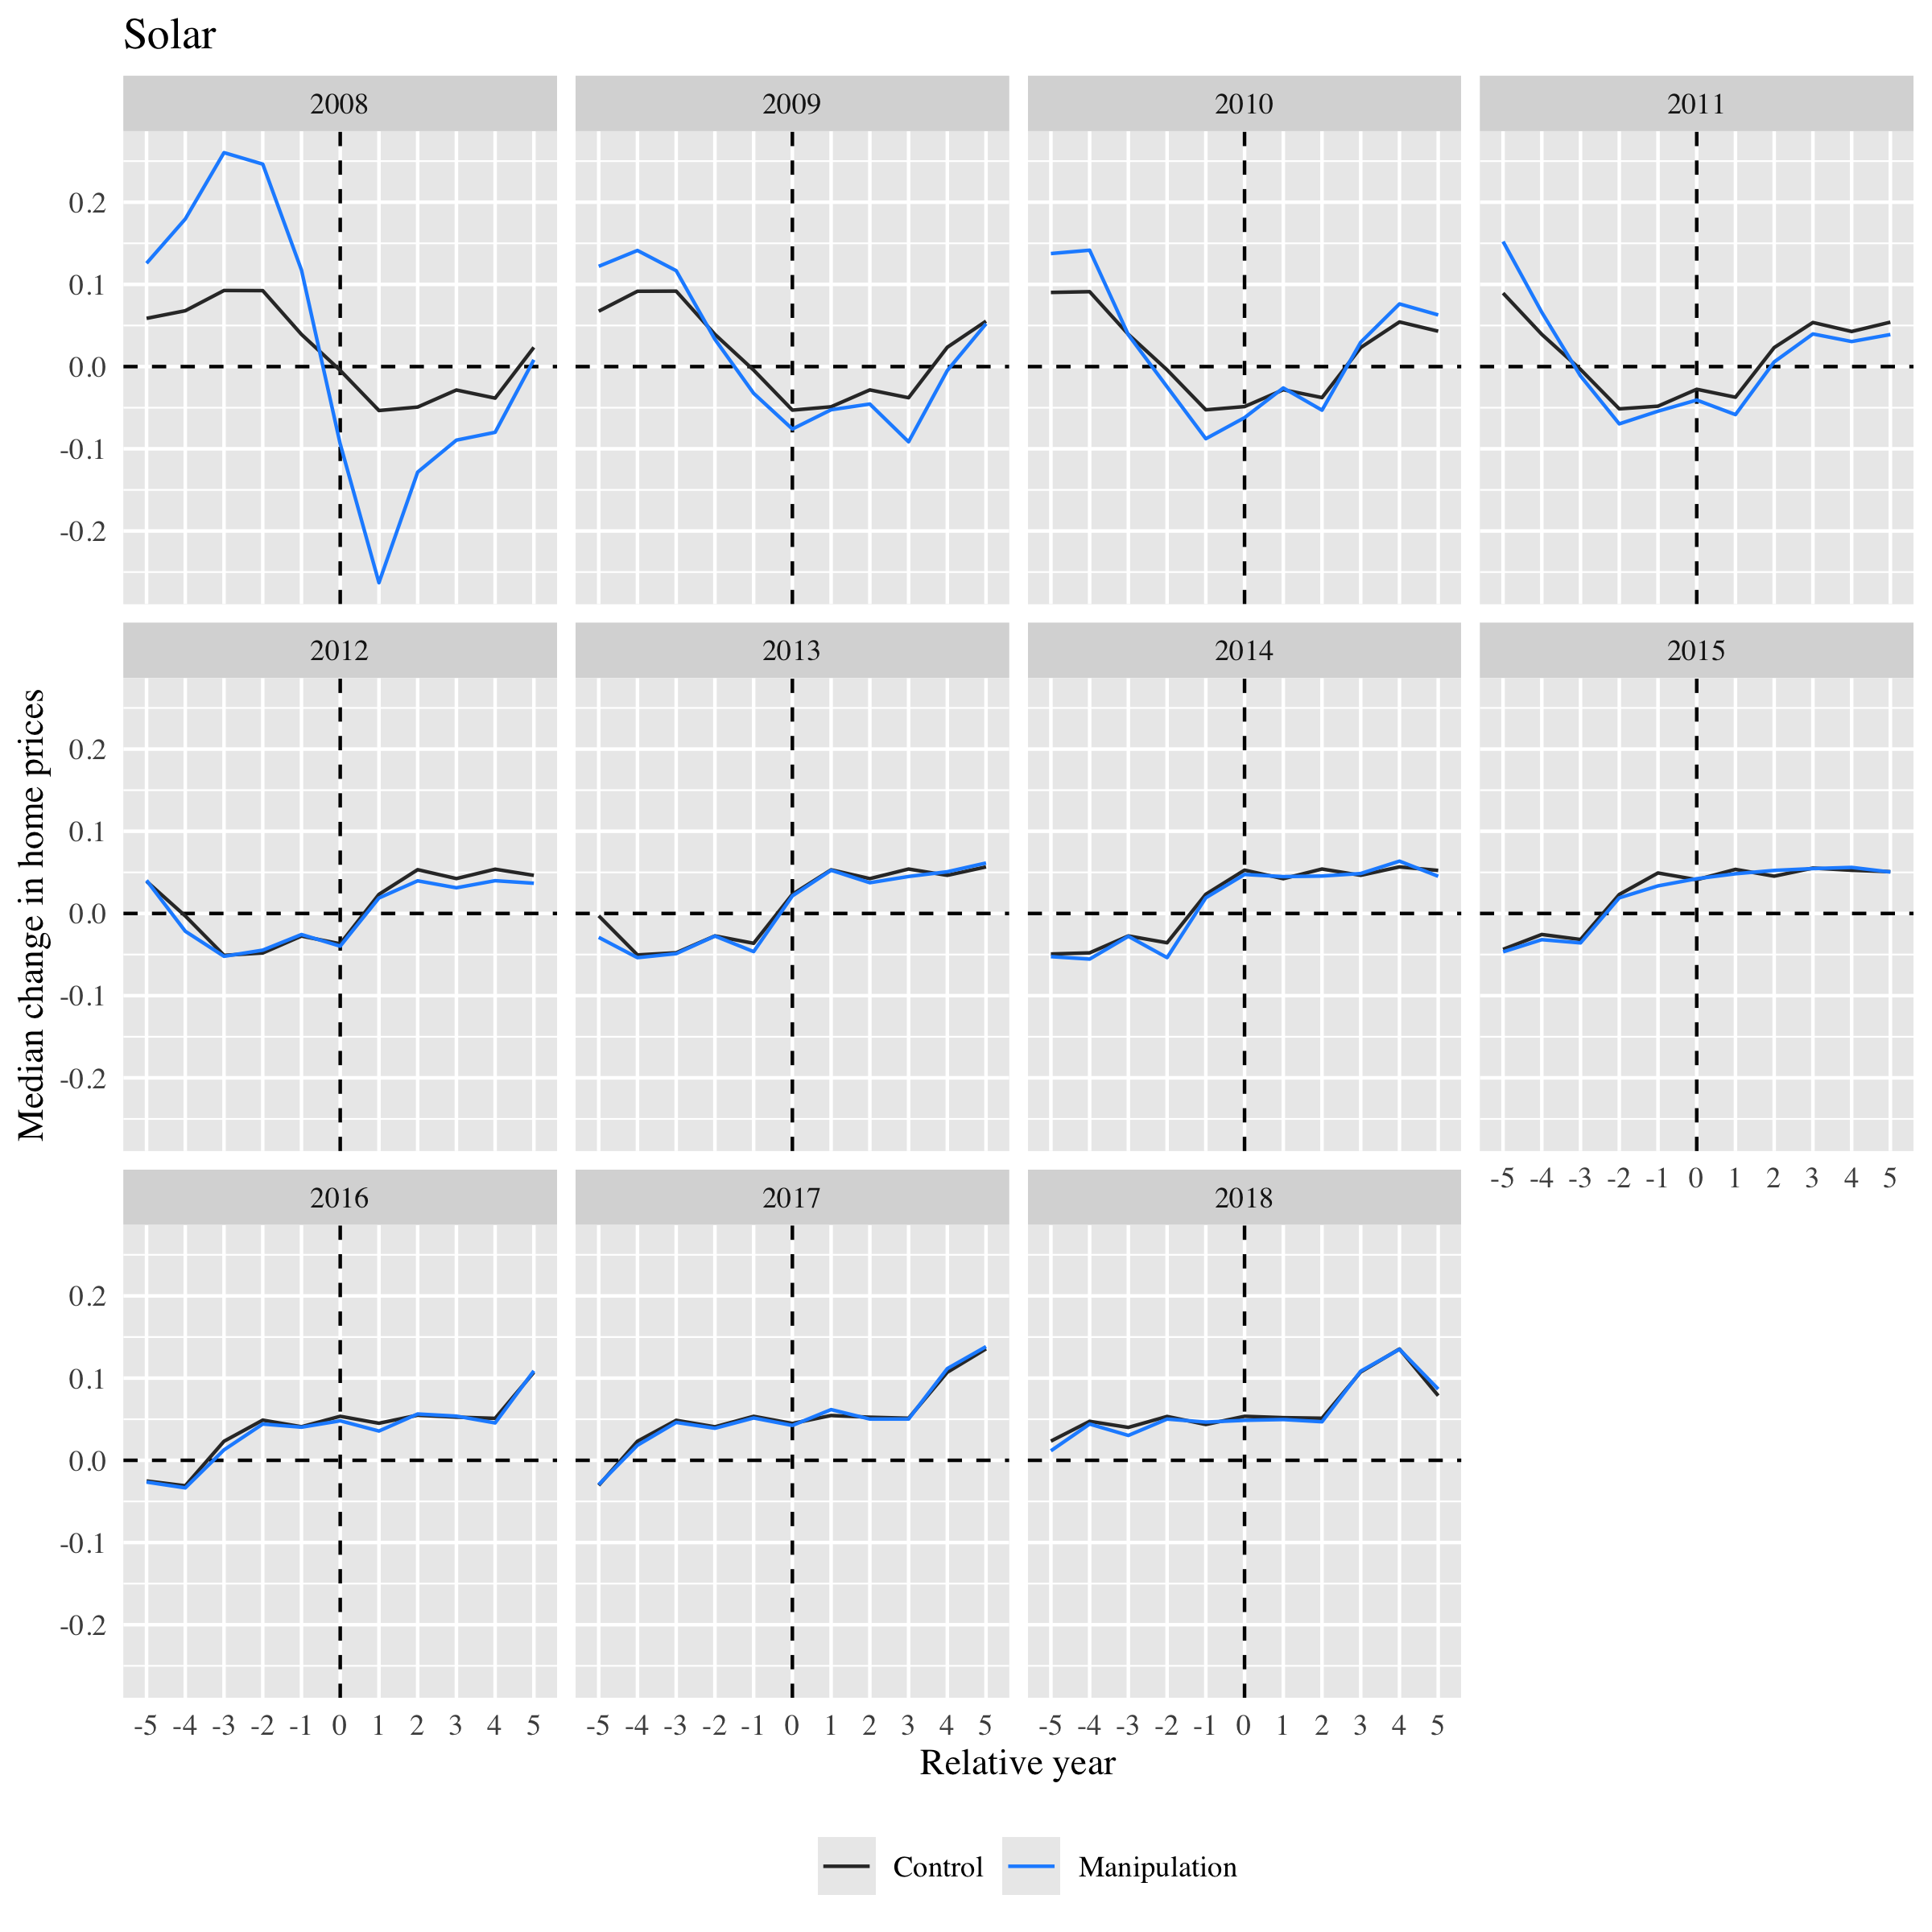
\includegraphics[width=0.9\linewidth]
{study1_solar_facets.png} 
\caption{Median change in home prices in zip-codes that had solar panels installed}
\label{study1solarfacets}
\end{figure}

Unfortunately, I don't think there's many lessons to glean from these diagrams, because they \emph{doesn't account for general changes in the real estate market.}
For example, we can see the market tanking in 2008, but this completely confounds our ability to compare these lines to those a decade later.
Figure\ref{study1turbinefacets} shows us the DiD for turbine facilities, but it suffers from the same shortcomings as figure\ref{study1solarfacets}.
\begin{figure}[h]
\centering
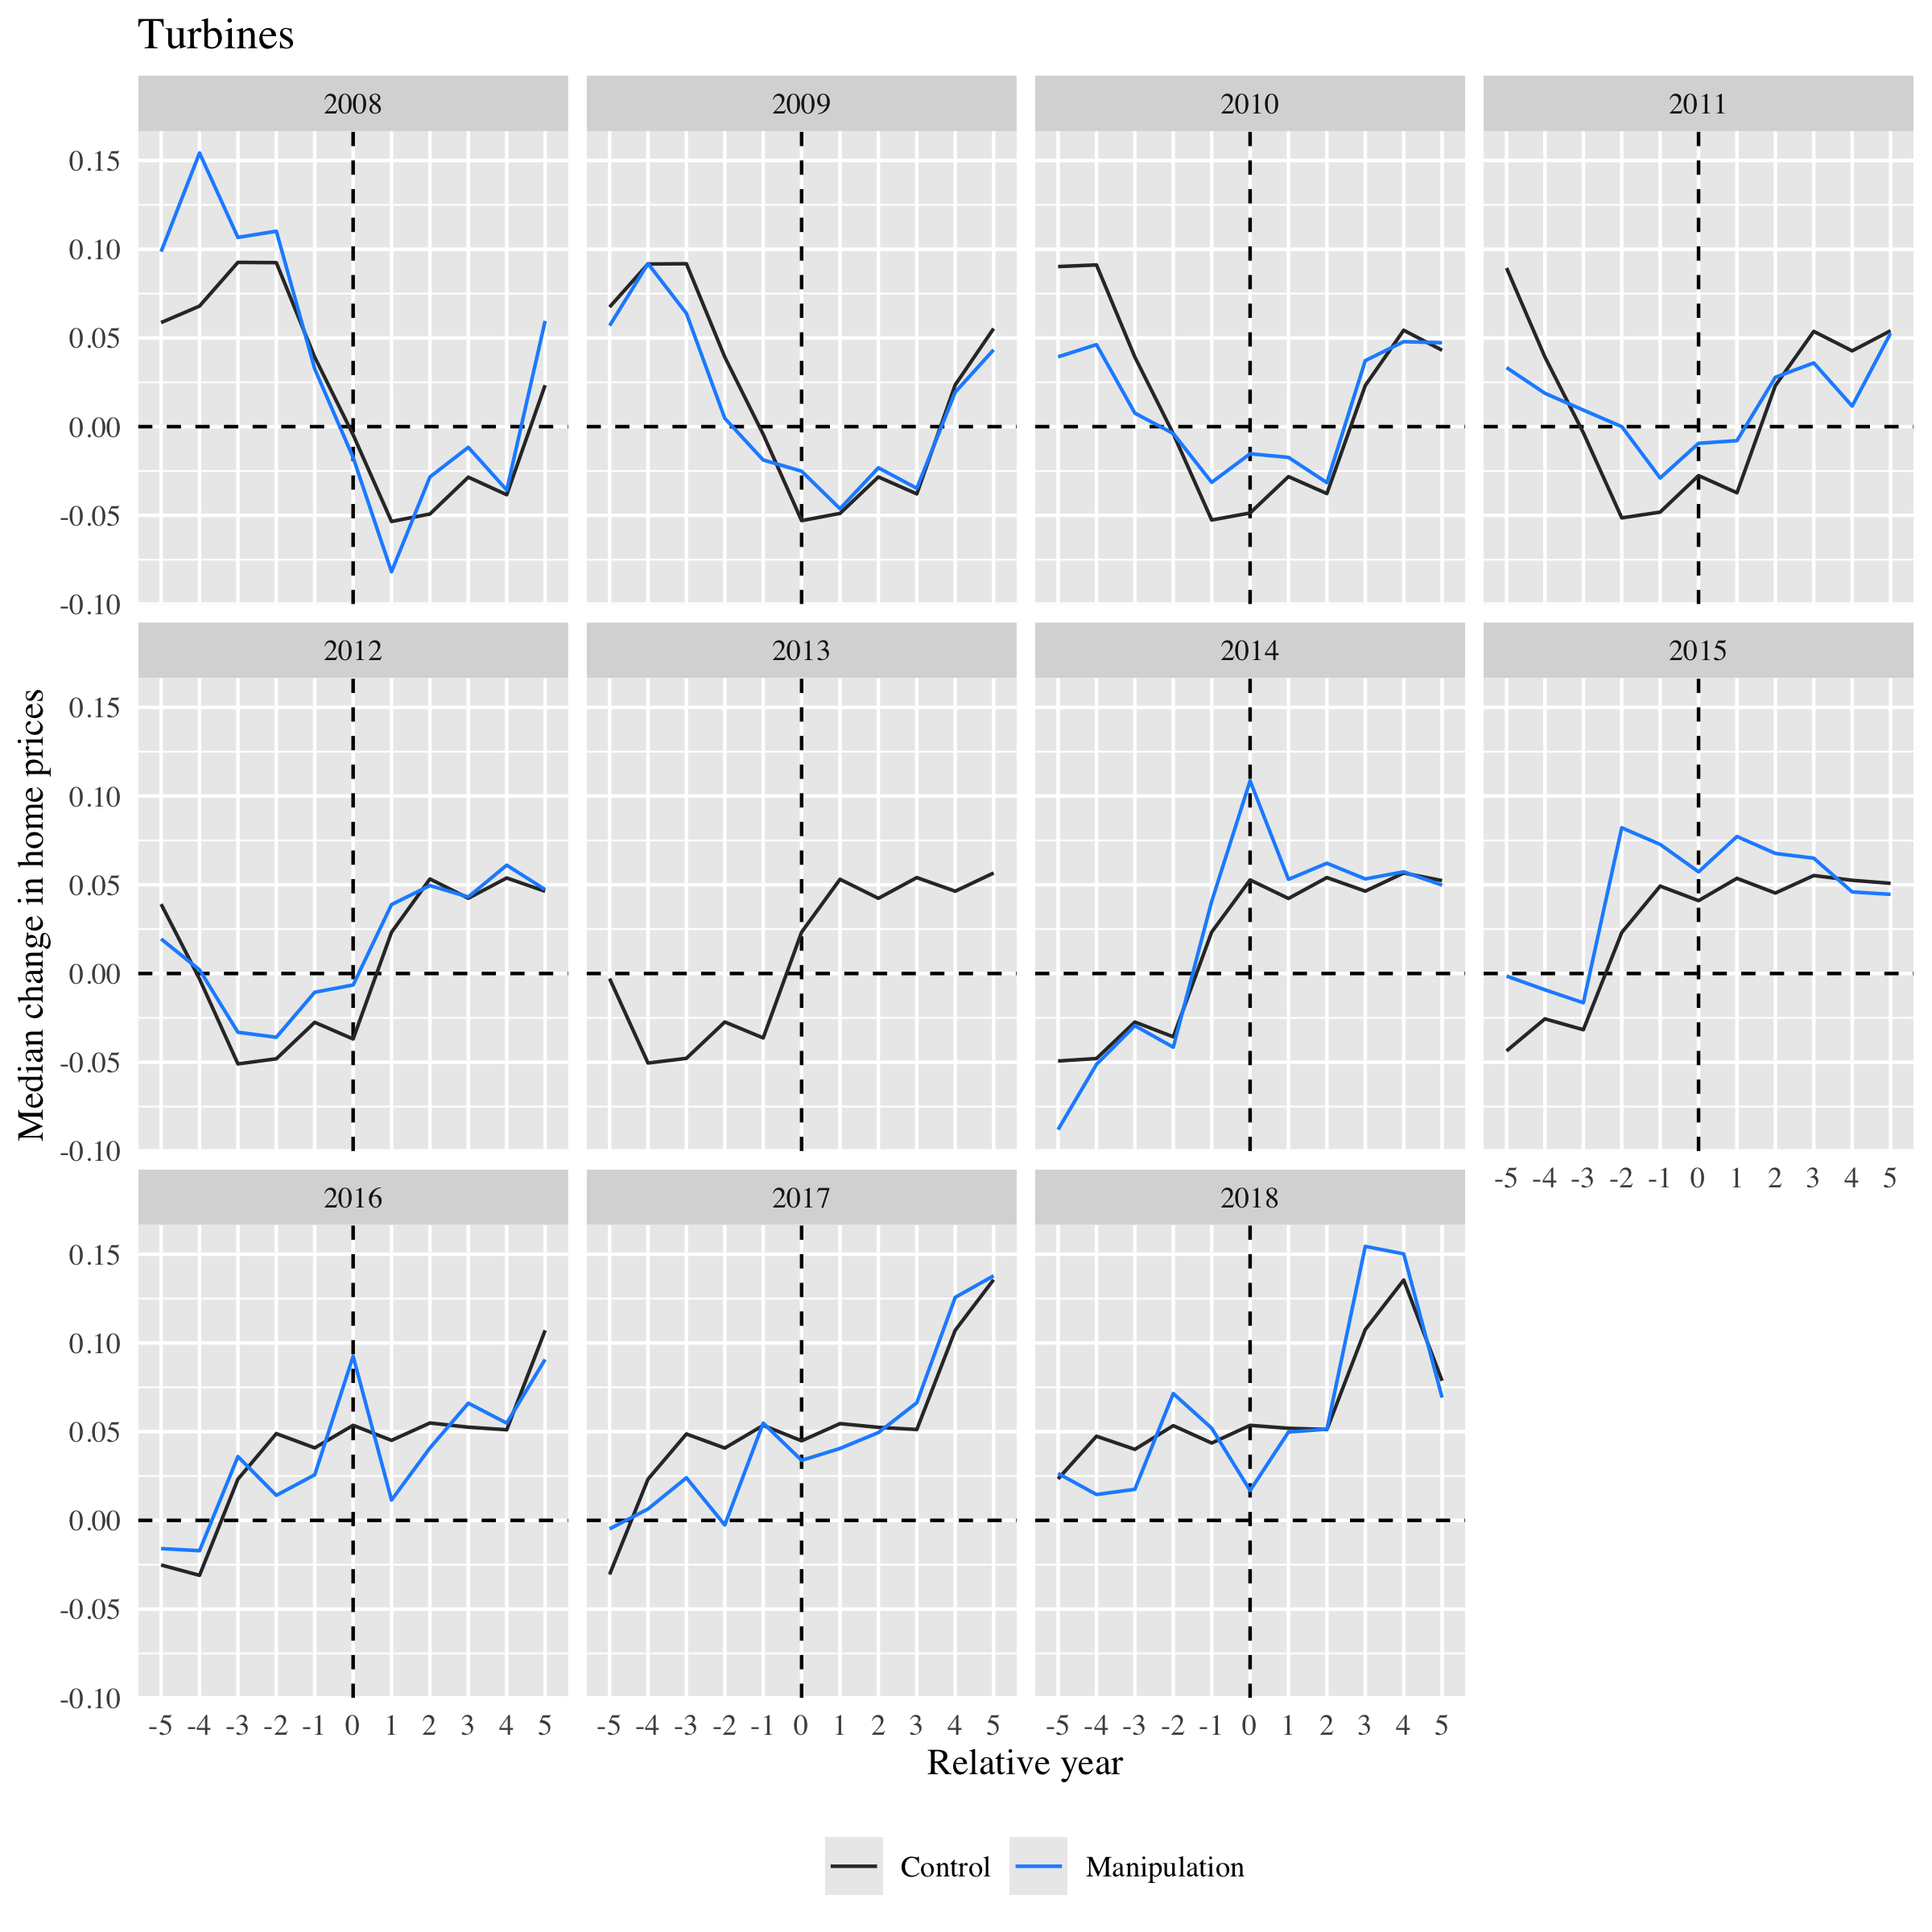
\includegraphics[width=0.9\linewidth]
{study1_turbine_facets.png} 
\caption{Median change in home prices in zip-codes that had wind turbines installed}
\label{study1turbinefacets}
\end{figure}

The other issue with this DiD study is, once again, a small sample size (see figure \ref{study1samplesize}). 
The sample sizes for the manipulation groups pictured here are very small, only a fraction of the size of the control group.
In addition to this problem, while the observations in the manipulation group change in each of the diagrams, the observations in the control group stay the same.
This means that individual outliers in the control group might be skewing our results.
\begin{figure}[h]
\centering
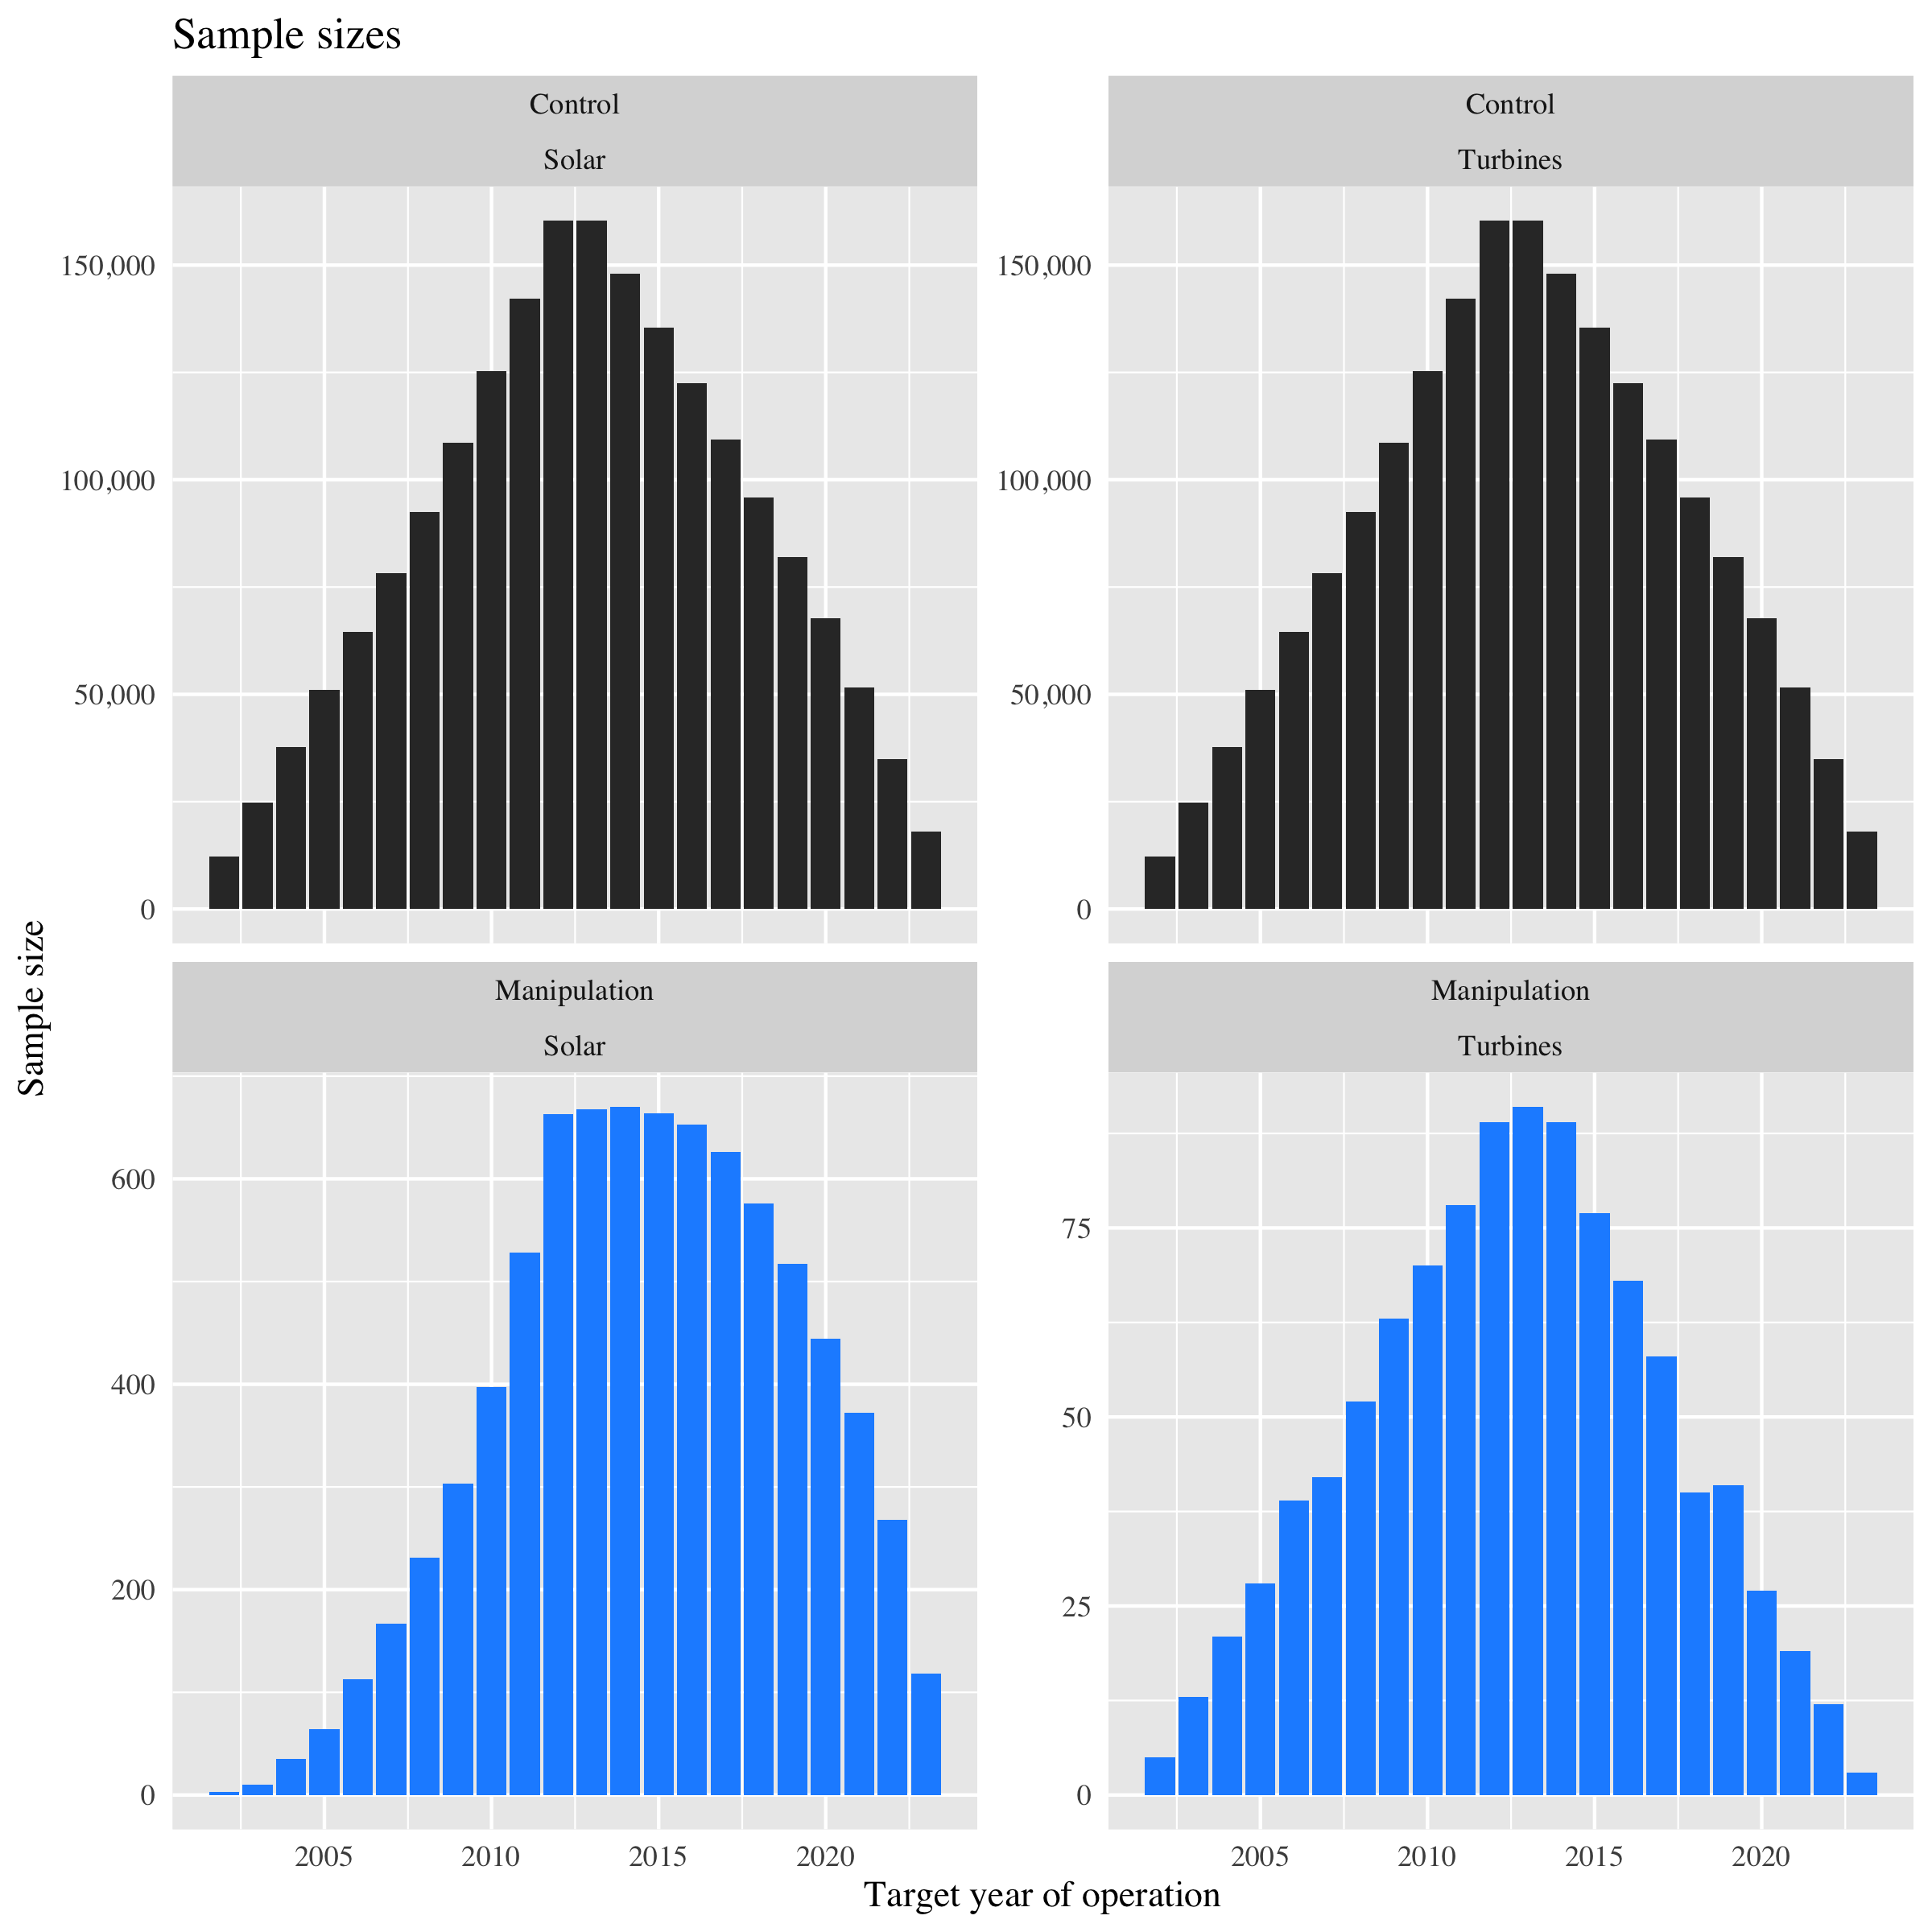
\includegraphics[width=0.9\linewidth]
{study1_sample_size.png} 
\caption{The manipulation groups in the DiD study were extremely small}
\label{study1samplesize}
\end{figure}

\end{document}
